\documentclass[11pt]{article}
\usepackage{amsmath, fullpage, parskip, graphicx}

\begin{document}
\title{DS Coursework}
\author{Jacob Essex \\ s1040340}
\maketitle

\subsection*{Q1}

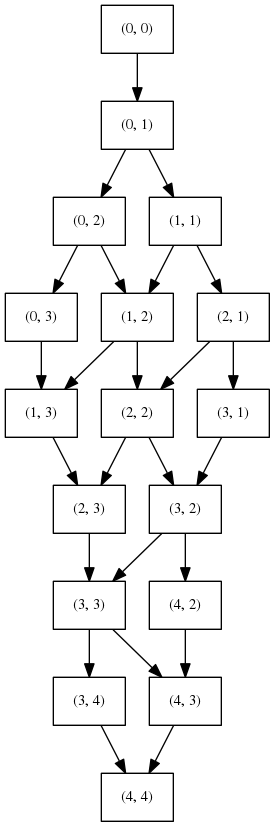
\includegraphics[width=0.3\textwidth]{q1_theory.png}


\subsection*{Q2}
To avoid starvation an alogirthm needs to be fair (i.e. requests for a lock are honored in the order that they are made). This prevents starvation. A system that is libable to have starvation is one that always grants the request of the most recent request.

\subsection*{Q3}

Data is trasnfered between nodes. This data is of fixed size and is represented using the following tuple
$$
(\text{sum of all p.f seen}, \text{max of all p.f seen}, \text{number of processors seen})
$$

The algorithm is as follows:

Each leaf sends its $(p.f, p.f, 1)$ to its parent

On recipt of all data $(sum_i, max_i, count_i)$ from its $i$th of $n$ children each node p sends the following data to its parents unless it is the root node in which case it does nothing
$$(p.f + \sum_i^n sum_i, \text{MAX}(p.f, max_1, max_2, ... max_n), 1 + \sum_i^n count_i)$$

The root node will then hold $(\text{sum}, \text{max}, \text{count})$
It then preforms the following operation on its tuple to product a new tuple 
$$(\text{avg}, \text{max}) = (\text{sum/count}, \text{max})$$
This new tuple now contains the needed result.

The message length is fixed, so the cost of sending a message is fixed.
In the worst case, the minimum spanning tree represents a single line of processors.
In this case O(n) messages need to be sent taking O(n) time as the cost to send a message is fixed.

\subsection*{Q4}
The diameter of the network is defined by the longest shourtest path. In the case
the diameter of the weighted graph this is:
$d \rightarrow h \rightarrow l \rightarrow m$

If each edge had a weight of 1 then the following paths of cost 5 would realise this:
$ e \rightarrow a \rightarrow c \rightarrow g \rightarrow l \rightarrow m$ and
$e \rightarrow a \rightarrow c \rightarrow f \rightarrow i \rightarrow k$

Of course in both cases as the graph is undirected the reverse paths would also give the same results

\end{document}
